% Chapter 6

\chapter{Implementación} % Main chapter title

\label{Chapter6} % Change X to a consecutive number; for referencing this chapter elsewhere, use \ref{ChapterX}

En este Capítulo se explica la implementación del modelo de sistema propuesto en el Capítulo \ref{Chapter5}, para garantizar la fiabilidad de los resultados que generará el simulador, en este capítulo se realizan escenarios de prueba a cada uno de los modelos que comprende el simulador, se muestran resultados específicos por cada modelo y por último, se propone una metodología en cómo interconectar estos modelos. \ldots

%----------------------------------------------------------------------------------------
%	SECTION 
%----------------------------------------------------------------------------------------

\section{Generación de una geometría estocastica}

Generación de Puntos de Poisson en un círculo: \newline

Para una generación de puntos en un círculo correcta que cumpla con la definición de un HPPP [Sección \ref{PPP_C4}], el número total de puntos que se dibujarán en el círculo deberán ser una variable aleatoria de Poisson, además, estos puntos se deberán distribuir de acuerdo a una distribución uniforme dentro del círculo, por último, al considerar un proceso homogéneo, la densidad de los puntos será constante.\newline

Número total de puntos:\newline

En primer lugar, para cumplir con la definición de HPPP, el número total de puntos tendrá que seguir una distribución de Poisson. Para esto en cada realización se generará una variable aleatoria de Poisson con tasa constante $\lambda$ y media $\lambda A$ donde $A=\pi r^{2}$. \newline

Ubicación de los puntos:\newline

Después, para la distribución uniforme de puntos en un círculo, se consideraron dos variables aleatorias uniformes, una que represente el radio y otra el ángulo (esto con base en las coordenadas polares).\newline

Por otra parte, debido a que el área aumenta de manera cuadrática con relación al radio, un punto aleatorio ubicado uniformemente en un círculo de radio $r$ tiene las coordenadas polares $[r(\sqrt{U}), 2\pi V]$, donde U y V son las dos variables aleatorias uniformes independientes, $U, V \in{[0,1]}$.

\subsection{Escenario de Prueba}

En este escenario se validó la generación de puntos siguiendo un HPPP.\newline

Para el primer caso en el número total de puntos que sigue una distribución discreta de Poisson, se comprobó la generación de la variable aleatoria Poisson en Python usando la libreria \textit{scipy}.\newline

Para esto, se realizaron $1000$ generaciones de numeros siguiendo una distribución de Poisson con tasa $\lambda = 1000$, se obtuvo el histograma de todos los números generados y se comparó con su función de masa de probabilidad (PMF).\newline

Se observa que la distribución del histograma sigue a la función masa de probabilidad de Poisson [\textit{véase Figura~\ref{fig:generacionPoisson}}], por lo que se valida la generación de números Poisson en Python.\newline

\begin{figure}[th]
    \centering
    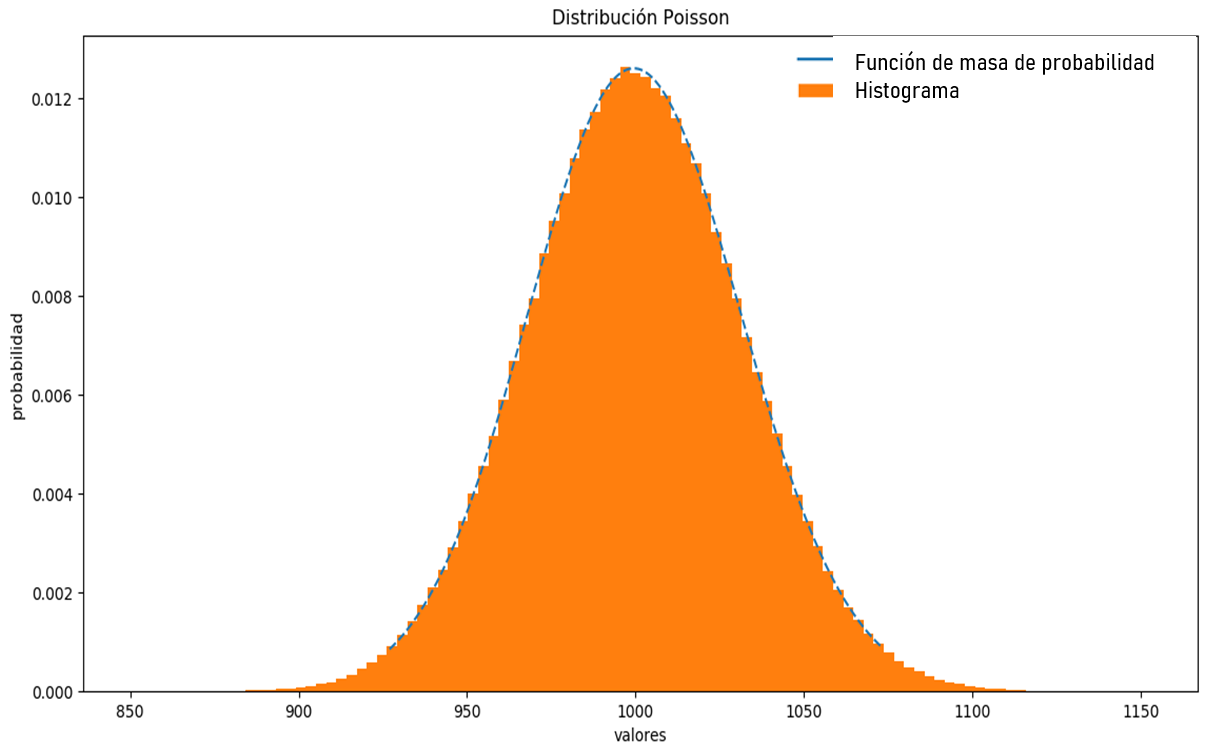
\includegraphics[scale=.4]{Figures/PoissonDistribution}
    \decoRule
    \caption[Gráfica comparación PMF e histograma de distribución Poisson en Python]{Gráfica comparación PMF e histograma de distribución Poisson en Python}
    \label{fig:generacionPoisson}
\end{figure}

También, se comprobó la generación de puntos aleatorio ubicados uniformemente en un círculo de radio $r$ en coordenadas polares $[r(\sqrt{U}), 2\pi V]$.\newline

Se graficó en un círculo 2D la generación de puntos, con tasa constante $\lambda = $ y media $\lambda A$ donde $A=\pi r^{2}$ donde $r = $.

Por último, se validó que todos los puntos se generen dentro del areá del circulo, para esto se graficó de igual manera la distribución espacial de los puntos en un círculo en plano 2D pero ahora con una densidad mayor, de modo que se observe que los puntos rellenan toda el área del círculo [\textit{véanse Figuras~\ref{fig:PPPCirculo1}, \ref{fig:PPPCirculo2}}].

\begin{figure}
    \centering
    \begin{minipage}{.45\linewidth}
      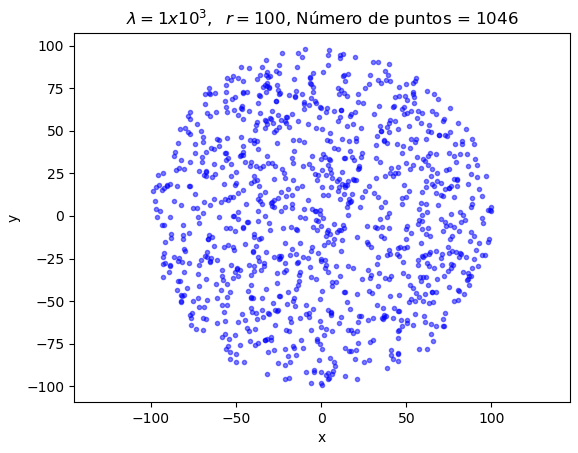
\includegraphics[width=\linewidth]{PPPCirculo1}
      \caption[Distribución espacial de puntos PPP en un círculo 2D]{Distribución espacial de puntos PPP con media $\lambda A$ en un círculo 2D}
      \label{fig:PPPCirculo1}
    \end{minipage}
    \hspace{.05\linewidth}
    \begin{minipage}{.45\linewidth}
      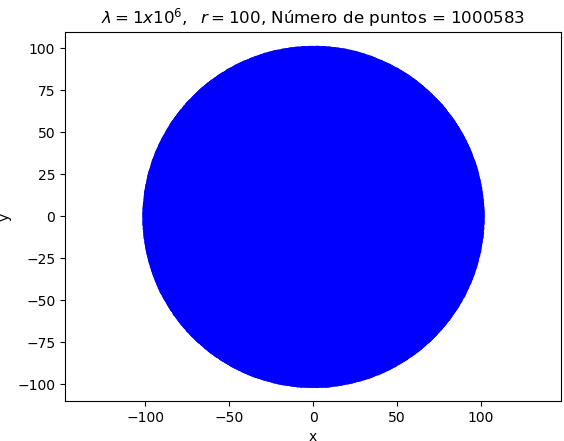
\includegraphics[width=\linewidth]{PPPCirculo2}
      \caption[Distribución espacial de puntos PPP en un círculo 2D]{Distribución espacial de puntos PPP con media $\lambda A$ en un círculo 2D}
      \label{fig:PPPCirculo2}
    \end{minipage}
\end{figure}


%----------------------------------------------------------------------------------------
%	SECTION 
%----------------------------------------------------------------------------------------

\section{Generación de ganancias de canal implementando pérdidas por distancia (PLE) y desvanecimiento Rayleigh}

De acuerdo con el modelo de canal propuesto, el modelo CI \textit{Ecuación~\ref{eqn:CI}} \parencite{Sun2016}, este implementa pérdidas de acuerdo con la distancia, dado un exponente de pérdida por trayectoria (PLE) y agrega pérdidas por el desvanecimiento rápido de Rayleigh.\newline

Cuando se habla del desvanecimiento de Rayleigh en enlaces inalambricos, en la literatura \parencite{RayleighScienceDirect} se encuentra que las componentes en cuadratura y en fase de la señal recibida son variables aleatorias Gaussianas con media cero que se distribuyen de forma independiente e idéntica (iid), siendo así, que la magnitud de la señal banda base compleja sigue una distribución de Rayleigh. Por otra parte, la distribución de la potencia normalizada de una señal de banda base compleja recibida bajo el desvanecimiento unitario de Rayleigh es modelado por medio de una distribución exponencial unitaria.\newline

Por lo tanto, cuando el desvanecimiento es Rayleigh, la magnitud (voltaje) de la señal es distribuida por Rayleigh pero su potencia es distribuida exponencialmente.\newline

En nuestro caso, como se trabajará en términos de potencia, se modelará este fenómeno por medio de la generación de una variable aleatoria que siga una distribución exponencial negativa con media unitaria, es decir, para cada $x>=0$ :

\begin{equation}
    f(x)=\lambda e^{-\lambda x}
\end{equation}
    $donde\ \lambda \to 1$

\subsection{Escenario de Prueba del desvanecimiento tipo Rayleigh en potencia}

Entonces, dado que en la generación de las ganancias Rayleigh se implementa la distribución continua Exponencial con media unitaria, se comprobó la generación de esta variable aleatoria en Python usando la libreria \textit{random}.\newline

Se realizaron $100000$ generaciones de numeros siguiendo una distribución Exponencial negativa con media $1$, se obtuvo el histograma de todos los números generados y se comparó con su función de densidad de probabilidad (PDF).\newline

Se observa que la distribución del histograma sigue a la función densidad de probabilidad Exponencial [\textit{véase Figura~\ref{fig:generacionExpon}}], por lo que se valida la generación de números Exponenciales en Python.\newline

\begin{figure}[th]
    \centering
    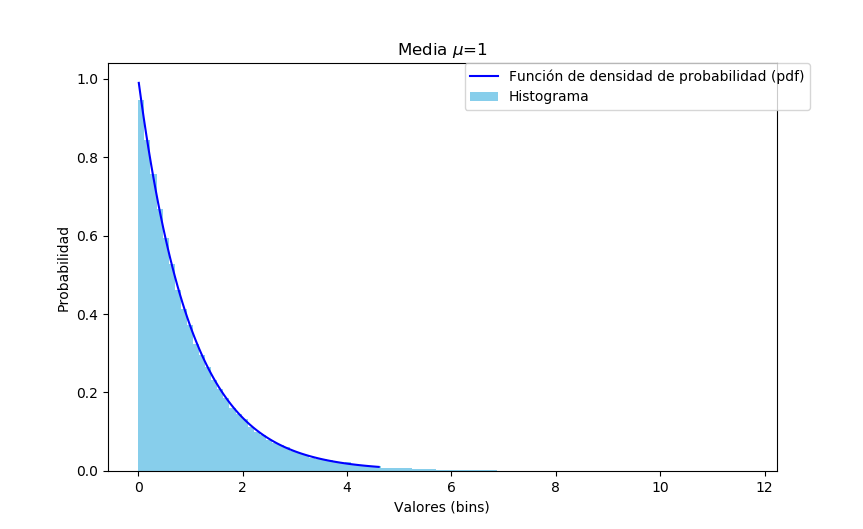
\includegraphics[scale=.7]{Figures/ExponentialDisitribution}
    \decoRule
    \caption[Gráfica comparación PDF e histograma de distribución Exponencial en Python]{Gráfica comparación PDF e histograma de distribución Exponencial en Python}
    \label{fig:generacionExpon}
\end{figure}
%\begin{figure}[th]
%    \centering
%    \includegraphics[scale=.6]{Figures/}
%    \decoRule
%    \caption[]{}
%    \label{fig:}
%\end{figure}
%----------------------------------------------------------------------------------------
%	SECTION 
%----------------------------------------------------------------------------------------

\section{Esquema de acceso múltiple al medio no ortogonal, basado en potencia (PD-NOMA)}

De acuerdo con el modelo de sistema (sección~\ref{}), se propuso implementar un esquema de acceso múltiple no ortogonal (NOMA), con base en \parencite{Shahini2019}, los autores desarrollaron un esquema NOMA basado en NB-IoT por medio de un agrupamiento óptimo de los usuarios y una optimización en la asignación de recursos, de acuerdo con la maximización de la tasa de transmisión total de subida de los dispositivos MTC.\newline

\subsection{Algoritmo de Agrupación de dispositivos uRLLC  y mMTC}

Se implementó el algoritmo de agrupamiento NOMA para los dispositivos mMTC y uRLLC descrito en \parencite{Shahini2019}[\textit{véase Algorithm \ref{A1}}], este algoritmo realiza un ordenamiento conveniente con respecto al uso de la Cancelación Sucesiva de Interferencia (SIC), es decir, se ordenan los dispositivos URLLC y mMTC de acuerdo con su ganancia de canal promedio dentro de los diferentes grupos NOMA para que puedan compartir el mismo recurso espectral (subportadora) asignado a cada grupo[\textit{Véase Figura~\ref{fig:NOMAgrupoexample}}].\newline

Por lo tanto, un mensaje combinado de los dispositivos mMTC y uRLLC con ruido aditivo es recibido en la BS, la BS emplea la recepción SIC de acuerdo en cómo son ordenados los dispositivos. \newline

La recepción SIC decodifica primero el mensaje del dispositivo con el rango más bajo, por consiguiente los usuarios con los rangos siguientes (o más altos) le introducen interferencia y a su vez el usuario con el rango más alto no experimenta interferencia de ninguna señal.\newline

\begin{figure}[th]
    \centering
    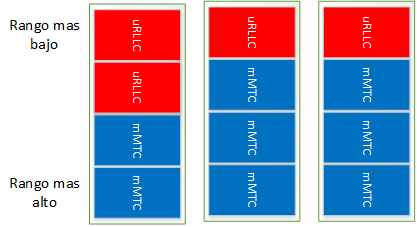
\includegraphics[scale=1]{Figures/EjemploNOMAclusters}
    \decoRule
    \caption[Ejemplo ilustrativo del ordenamiento de usuarios en los grupos NOMA]{Ejemplo ilustrativo del ordenamiento de 4 usuarios uRLLC y 8 usuarios mMTC en 3 grupos NOMA}
    \label{fig:NOMAgrupoexample}
\end{figure}

Es importante notar que los dispositivos uRLLC tienen requerimientos de tasas de datos más altos, por lo tanto, su potencia de transmisión será mayor que la de los dispositivos mMTC. Es por esto que en cada grupo los dispositivos uRLLC tendrán los rangos más bajos y los dispositivos mMTC los mas altos. De hecho, el decodificador SIC en la BS comienza a decodificar con URLLC y, en consecuencia, los dispositivos mMTC no se ven afectados por la alta interferencia de los URLLC [véase Figura XXX].\newline


%%%%%%%%%%%%%%%%%%%%%%%%%%%%%%%%%%%%%%%%%%%%%%%%%%%%%%%%       EJEMPLO DE ALGORITMO EN LaTeX       %%%%%%%%%%%%%%%%%%%%%%%%%%%%%%%%%%%%%%%%%%%%%%%%%%%%%%%%%%%%%
Definición de variables de los algoritmos 1 y 2:\newline

\begin{itemize}
    \item U: Lista de dispositivos uRLLC
    \item M: Lista de dispositivoss mMTC
    \item S: Lista de Subportadoras s
    \item C: Lista de Grupos NOMA
    \item $R_{m}^{th}:$ Tasa objetivo del enésimo dispositivo m mMTC 
    \item $R_{u}^{th}:$ Tasa objetivo del enésimo dispositivo u uRLLC
    \item $P_{m}^{max}:$ Potencia máxima del enésimo dispositivo m mMTC 
    \item $P_{u}^{max}:$ Potencia máxima del enésimo dispositivo u uRLLC (i.e. 23dBm)
    \item $P_{m}^{s}:$ Potencia del enésimo dispositivo m mMTC 
    \item $P_{u}^{s}:$ Potencia del enésimo dispositivo u uRLLC 
    \item $h_{m}^{s}:$ Ganancia de canal del enésimo dispositivo m mMTC sobre la portadora s
    \item $h_{u}^{s}:$ Ganancia de canal del enésimo dispositivo u uRLLC sobre la portadora s
    \item ${\hat S}$: Lista de subportadoras asignadas
    \item $S_{a}^{c}$: Lista de subportadoras asignadas al enésimo cluster
    \item ${C_{ns}}$: Lista de cluster aún no asignados
\end{itemize}


\makeatletter
% Reinsert missing \algbackskip
\def\algbackskip{\hskip-\ALG@thistlm}
\makeatother

\begin{algorithm}
    \caption{Algoritmo de agrupamiento de dispositivos uRLLC y mMTC para NOMA}\label{A1}
    \hspace*{\algorithmicindent} \textbf{Entrada} $U, M, S, C, h_{m}^{s} , \ and \ h_{u}^{s} ,\forall m \in \mathcal {M} , \forall u \in \mathcal {U} , \forall s \in \mathcal {S}$  \\
    \hspace*{\algorithmicindent} \textbf{Salida} Lista de Clusters (C) con agrupamiento de dispositivos 
    \begin{algorithmic}[1]
    \Procedure{Agrupación de dispositivos uRLLC}{}\\
    Cálculo de la ganancia de canal promedio del enésimo dispositivo u\\
    ${\tilde h_{u}} =\sum \nolimits _{s \in \mathcal {S}} {h_{u}^{s}}{/_{|S|}}$\\
    Se ordenan descendentemente las ganancias de canal promedio de cada dispositivo u, i.e. $\forall u \in \mathcal {U} : {\tilde h_{1}} \geq {\tilde h_{2}} \geq \cdots \geq {\tilde h_{U}}$ 
    \For{\textbf{each} u in U}
        \If {$|U|<|C|$} 
        \State Asignar uRLLC al rango mas bajo (k=1)
        \Else
        \State Asignar uRLLC al siguiente rango (k=2) [Solo se podrán asignar hasta un segundo rango]
        \EndIf
    \EndFor
    \State Encontrar ${\tilde k}$, rango y grupo en el que se quedó la última asignación uRLLC
    \EndProcedure
    \Procedure{Agrupación de dispositivos mMTC}{${\tilde k}$}\\
    Cálculo de la ganancia de canal promedio del enésimo dispositivo u\\
    ${\tilde h_{m}} =\sum \nolimits _{s \in \mathcal {S}} {h_{m}^{s}}{/_{|S|}}$\\
    Se ordenan descendentemente las ganancias de canal promedio de cada dispositivo u, i.e. $\forall m \in \mathcal {M} : {\tilde h_{1}} \geq {\tilde h_{2}} \geq \cdots \geq {\tilde h_{M}}$ 
    \For{\textbf{each} m in M}
        \If {$|M|<|C|$} 
        \State Asignar mMTC al rango ${\tilde k}$
        \Else
        \State Asignar mMTC a los siguientes rangos \ldots
        \EndIf
    \EndFor
    \EndProcedure
    \end{algorithmic}
\end{algorithm}


\subsection{Algoritmo de Asignacion de Subportadoras}

Este algoritmo garantiza una óptima asignación de portadoras (S), de acuerdo con la maximización de la tasa total de transmisión, para los grupos NOMA. En \parencite{Shahini2019} se plantea la metodología para la asignación de subportadoras. \newline

Cabe destacar que en \parencite{Shahini2019}, el modelo de sistema no es implementado hacia una banda de frecuencias en específico, por lo que las subportadoras S son una variable aleatoria dentro de su simulación.\newline

Para cada subportadora, el mejor grupo (c*) es el que maximiza el rendimiento total, [\textit{véase Algorithm \ref{A2}}]. Luego, por consecuencia, las velocidades de datos de los dispositivos mMTC y URLLC y sus potencias de transmisión se actualizan. Durante el proceso de asignación de subportadoras, los clústeres asignados se excluyen del conjunto de Cns. \newline

El algoritmo asigna iterativamente las subportadoras una por una. Dado que cada dispositivo MTC divide por igual su potencia de transmisión máxima entre todas las subportadoras asignados, las potencias de transmisión de los dispositivos MTC a través de las diferentes subportadoras no son óptimas utilizando el algoritmo planteado. \newline

La fase de asignación de recursos termina hasta que las 48 subportadoras se asignan a los 48 clústeres NOMA. \newline

%ESTO VA DESPUÉS
Los autores en \parencite{Shahini2019} proponen la oportunidad de asignar más de una subportadora (\textit{multitone}) por grupo NOMA en transmisiones con anchos de banda UL de 3.75KHz para NB-IoT. Entonces, aunque aún no ha sido especificado la asignación de múltiples subportadoras por cluster en anchos de banda de 3.75KHz para NB-IoT, se tomó la propuesta de \parencite{Shahini2019} en este simulador. \newline

No se satisfacen todos los requisitos de velocidad de datos de los dispositivos mMTC y URLLC pero si se incrementa significativamente la conectividad de usuarios en comparación con SC-FDMA donde solo se puede dar servicio a un usuario por subportadora, es decir, en total a 48 usuarios.\newline


\begin{algorithm}
    \caption{Algoritmo de asignación de recursos para NOMA}\label{A2}
    \hspace*{\algorithmicindent} \textbf{Entrada} $U, M, S, C , R_{m}^{th} , R_{u}^{th} , P_{m}^{max} , P_{u}^{max} , h_{m}^{s} , \ and \ h_{u}^{s} ,\forall m \in \mathcal {M} , \forall u \in \mathcal {U} , \forall s \in \mathcal {S}$  \\
    \hspace*{\algorithmicindent} \textbf{Salida} Asignaciones de grupos con subportadoras (Asignación de todas las subportadoras [48, NB-IoT singletone]) 
    \begin{algorithmic}[1]
    \Procedure{Asignación de subportadoras}{}\\
    $Inicialización: $ \\${R_{u}} = 0 , {R_{m}} = 0 , p_{m}^{s}=P_{m}^{max} \ y \ p_{u}^{s}= P_{u}^{max} , \forall m \in \mathcal {M} , \forall u \in \mathcal {U} , \forall s \in \mathcal {S}.$ 
    ${\hat S} \leftarrow \emptyset,~~S_{a}^{c} \leftarrow \emptyset,~~{C_{ns}} \leftarrow \mathcal {C}$ 
    \While{$\mathcal{S} \ne \emptyset$}{}
    \BState \emph{Asignación de una subportadora a un grupo NOMA}:
        \For{\textbf{each} s in S}{
        \State Seleccionar al mejor cluster $c^{*}$ (el que maximiza el throughput):
        \State ${c^{*}} = \mathop {\arg \max }\limits _{c \in {C_{ns}}} \left ({{\sum \nolimits _{u \in \mathcal {U}} {R_{u} + \sum \nolimits _{m \in \mathcal {M}} {R_{m}} } } }\right) ;$ 
        \State donde: Ru \textit{(Ecuación \ref{eqn:Ru})} y Rm \textit{(Ecuación \ref{eqn:Rm})}, de acuerdo con \parencite{Shahini2019}
        \State $Asignar\ la\ subportadora\ s\ con\ c^{*} :$ 
        \State $Actualizar\ S_{a}^{c^{*}}\ \leftarrow S_{a}^{c^{*}} \cup \{ s\} , \hat S \leftarrow \hat S \cup \{ s\}$ 
        \State $Actualizar\ las\ tasas: {R_{u}} = {R_{u}} + {R_{u,s}} ,\ {R_{m}} = {R_{m}} + {R_{m,s}}$ 
        \State $Actualizar\ las\ potencias\ de\ los\ URLLC\ y\ mMTC\ de\ c^{*}\ individualmente:$ 
        \State $p_{m}^{s} = \frac {p_{m}^{s}}{{\left |{ {S_{a}^{c^{*}}} }\right | + 1}} ,\ p_{u}^{s} = \frac {p_{u}^{s}}{{\left |{ {S_{a}^{c^{*}}} }\right | + 1}} , \forall s \in \mathcal {S}$ 
        \If {$ S_{a}^{c^{*}} == 1$}{
        \State ${C_{ns}} \leftarrow {C_{ns}}\backslash \{{c^{*}}\}$ 
        \EndIf}
        \EndFor}
    \EndWhile
    \BState \emph{Asignación de subportadoras restantes}:
    \If {$ C_{ns} \ne \emptyset $} { 
        \For{\textbf{each} s in S}{
            \State $\mathcal {S} \leftarrow \mathcal {S}\backslash \hat S$ 
            \State ${c^{*}} = \mathop {\arg \max }\limits _{c \in {C}} \left ({{\sum \nolimits _{u \in \mathcal {U}} {R_{u} + \sum \nolimits _{m \in \mathcal {M}} {R_{m}} } } }\right)$ 
            \State $Actualizar\ S_{a}^{c^{*}} \leftarrow S_{a}^{c^{*}} \cup \{ s\}$ 
        \EndFor}
            \State $Actualizar\ p_{m}^{s} = \frac {p_{m}^{s}}{{\left |{ {S_{a}^{c^{*}}} }\right | + 1}} ,\ p_{u}^{s} = \frac {p_{u}^{s}}{{\left |{ {S_{a}^{c^{*}}} }\right | + 1}}$ 
    \EndIf}
    \EndProcedure
    \end{algorithmic}
\end{algorithm}


\subsection{Escenario de Prueba de los Algoritmos 1 y 2}



%----------------------------------------------------------------------------------------
%	SECTION 
%----------------------------------------------------------------------------------------

\section{Generación de Tráfico Fuente}

\subsection{Tráfico CMMPP}
\subsection{Escenario de Prueba de Tráfico CMMPP}

%----------------------------------------------------------------------------------------
%	SECTION 
%----------------------------------------------------------------------------------------

\section{Interconexión de los 4 módulos del Simulador}
%Incluir lo de NPRACHH, NPUCSH y NORA

%----------------------------------------------------------------------------------------
%	SECTION 
%----------------------------------------------------------------------------------------

\section{Simulador de Eventos Discretos}

\subsection{Definición de eventos}

\subsection{Interfaz de usuario}

\subsection{Descripción de los \textit{logs} de salida}

%----------------------------------------------------------------------------------------
%	SECTION 
%----------------------------------------------------------------------------------------

\section{Optimización de tiempos de simulación}
